\documentclass[0-thesis.tex]{subfiles}

\begin{document}
The previous sections proposed the update architecture of the thesis, its key components,
and security considerations such as identity and access control. This section will discuss
a prototype implementation of the architecture as well as a manifest generator. 

\subsection{Prototype Design}
\label{ssec:prototype-design}
The prototype is developed as a means of evaluating the efficiency of the transport during
an update procedure. It consists of an update server and a client (device). The prototype
is using a pull model where the device initiates the update procedure. The notion of an
operator is cut out as it will not be used in a real deployment, as such there is only the
update server and client.

Contiki-NG, introduced in Section~\ref{sec:contiki-ng}, is the operating system of choice
for both the client and server. It is an operating system suitable for constrained devices
such as those of wireless sensor networks. Contiki-NG comes with a network stack featuring
CoAP(s) and DTLS which are the target protocols for the prototype. The reason for
implementing the update server prototype in Contiki-NG is as a proof of concept that a
more capable IoT device in a network could act as an update server. Of course, storage for
the firmware images hosted on the server must be accomodated for, a real deployment might
opt to use the Coffee filesystem together with Contiki-NG \parencite{coffee}. The server
prototype of this thesis will run as a native Contiki-NG process on a host computer (thus
using the computers' filesystem), while the client will be developed natively then ported
to a Firefly board.

The interactions of the client and server are simplistic and the client has no other
behaviour than to initialize and complete the update procedure. As shown in
Figure~\ref{fig:client-server-interaction}, the interaction starts with a POST request
from the client to the registration endpoint of the server. The registration is sent as a
confirmable CoAP packet and is thus acknowledged. Afterwards, the client sends a GET
request for a manifest. The idea is that the endpoint \texttt{update/manifest} is a well
known endpoint just like \texttt{update/register} and all devices in the network register
and poll for manifests at these endpoints. Upon a request to \texttt{update/manifest} it
is up to the server to decide whether there is a suitable manifest or not, the decision
making is offloaded from the device. The prototype only makes use of one manifest thus
such logic is not implemented, but in real deployments the \texttt{update/manifest}
resource would handle that (using the information from the devices' profile).

% TODO: Mention keys and certs for DTLS and COSE once it is figured out

\begin{figure}
    \caption{The interactions of client and server during an update procedure.}
    \label{fig:client-server-interaction}
    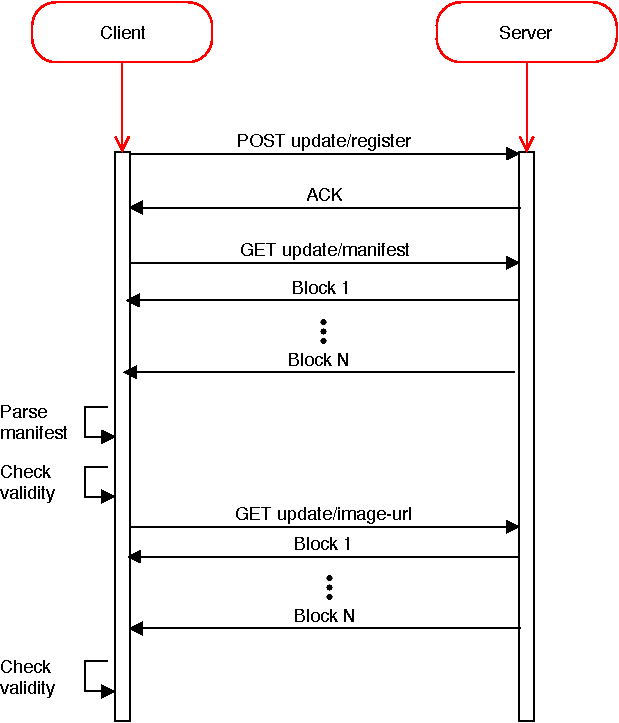
\includegraphics{images/client-server-sequence.pdf}
\end{figure}

If a suitable manifest is found, it is then transferred back to the client. As most
manifests will be too large for a single CoAP message, the server makes use of the block
option in CoAP. The manifest is split in chunks that are sent one by one. The client
receives these chunks and reassembles the manifest as it is received. After the manifest
in its entirety has been transferred, the client parses the manifest and checks its
validity by comparing vendor and class IDs. As described in
Section~\ref{ssec:manifest-format} there can be more preconditions requiring more checks,
again this is deployment specific. 

If the client deems the manifest to be valid it requests the update image from the URL
specified in the manifest. The endpoint is now specific for this particular class of
device and version and is not known in advance, it must be in the manifest. The image,
also too large for a single CoAP message, is transferred in blocks. When the client has
received the image, it calculates the SHA-256 hash of it, comparing it to the hash
contained in the manifest. This concludes the transfer of an update.

\subsection{Manifest Generation}
\label{ssec:manifest-generation}
As manifests contain certain information difficult for humans to provide such as
monotonically increasing sequence numbers and digests, a manifest generator was created to
help test the prototype \parencite{manifest-generator}. It is a Python script which
accepts information about vendor and class namespace, version, image, and associated URL
to generate, format, and output a manifest both in JSON and CBOR. The outputted manifest
follows the format specified in Section~\ref{ssec:manifest-format} and features all
required fields although many left blank. It is a bare-bones manifest containing only the
required information for a singular, monolithic update. There are no dependencies or
options. The example manifest used can be found in Appendix X. % TODO: Include example
manifest in appendix.

\end{document}